\section{State Estimator} \label{sec:state-estimator}

Following Charles' project, T-DAB employee Thomas Ryder carried on his work. Thomas' goal was to create a full pipeline which would create \emph{n} separate state estimator models, given the dataset in csv format.  Charles had worked on his project using Jupyter Notebooks. Thomas converted those notebooks into concise Python scripts, plus incorporated bayesian optimization into each of the \emph{n} models like Charles suggested as a future work. Thomas' scripts now consists of the following parts, explained very briefly below:

\begin{enumerate}
  \item \textbf{Preprocessing:} Rename and select columns, convert angles to radians, scale, label tacks, split into train-validation-test segments, and downsample the data.
  \item \textbf{Optimisation:} Run Bayesian optimization for each feature within the parameters given in the config file.
  \item \textbf{Training:} Train an LSTM network with optimized hyperparameters for each feature given in the config file. Log the training history data.
  \item \textbf{Evaluation:} Make predictions using the test data, then calculate MAE and RMSE. Print information about trained models.
\end{enumerate}

The scripts work as intended in local machines and Azure cloud machines. However, there are some problems and tests that need to be tackled before the final models that will be used for the Reinforcement Learning Environment can be produced. 

\subsection{Tack Detection and Datasets} \label{subsec:tack-detection-and-datasets}

Thomas' script do not find tacks in the given datasets. Instead, the script takes the tack information hardcoded in the config file. The problem is that the tack information is available in only one of the datasets. The information about the available datasets can be seen in Table \ref{tab:datasets}. Stanislas was the first to implement the tack detection models, and he achieved substantial improvement in his results after the tacks were removed. The better option to solve this problem would be to incorporate Stan's tack detection models into Thomas' script pipeline. But running the tack detection model for all datasets seperately, saving the tack information to be entered before running the scripts would also work.

\begin{table}[h]
\centering
\begin{tabular}{|l|l|l|l|l|c|}
\hline
\textbf{\begin{tabular}[c]{@{}c@{}}Dataset name\\(Race)\end{tabular}} & \textbf{Boat} & \textbf{\begin{tabular}[c]{@{}l@{}}Original\\Format\end{tabular}} & \textbf{\begin{tabular}[c]{@{}l@{}}Original\\Length(h)\end{tabular}} & \textbf{\begin{tabular}[c]{@{}l@{}}Cleaned\\Length(h)\end{tabular}} & \textbf{\begin{tabular}[c]{@{}l@{}}Tack\\Detection\end{tabular}} \\ \hline
RDR         & \multirow{3}{*}{Concise 8}    & .nkz \& .csv  & 16    & 16    & $\ballotx$        \\ \cline{1-1} \cline{3-6}
DHREAM 18   &                               & .log          & 64.5  & 64.5  & $\ballotx$        \\ \cline{1-1} \cline{3-6} 
Atlantic    &                               & .nkz          & 290.9 & 228.7 & $\ballotcheck$    \\ \hline
DHREAM 20   & VMB                           & .nkz          & 70    & 6     & $\ballotx$        \\ \hline
transat\_1  & Unknown 1                     & .nkz          & 383.5 & 63.3  & $\ballotx$        \\ \hline
\end{tabular}
\caption{Available Datasets}
\label{tab:datasets}
\end{table}

\subsection{Data Split Methods} \label{subsec:data-split-methods}

There are two proposed ways of splitting the available datasets into training, validation, and testing sets; named as \emph{Normal} and \emph{Segment} by Thomas.
The Normal split method allocates the first 60\% of the data to training, next 20\% to validation and the last 20\% to testing. The Segment split method on the other hand, first splits the dataset into continuous segments separated by unusable areas such as tacks. Then each of those segments are individually split into train-validation-test using 60-20-20 split and then concatenated together.

The data in the available datasets are logged chronologically. The nuance is that the weather and sea conditions change during the course of the races. In order to train the models on all the different sea and weather conditions, Charles has used the segment split method, as if he had used the normal split method, the models couldn't have been trained on the conditions present towards the end of the race.

Charles achieved good results using the segment split. However, one recent concern about segment split is whether it causes data leak. When using the segment split, the test data is not really held-out. The models are trained on data that is very similar to the ones used in validation and test sets. Therefore we cannot test the performance of the models on how they would perform on unseen data. Second supervisor of this project, Eric Topham suggested two sets of models to be created with segment and normal split methods. The resulting models will then be compared if there is a considerable difference in the performance results.

\section{RL Framework}
After the Background Research, the planned Reinforcement Learning framework to use was OpenAI's Spinning Up framework. They provide clean implementations of modern RL algorithms, and a basic interface to apply the algorithms to OpenAI Gym environments, then plot the results. However, OpenAI Spinning Up has some downsides and lack some important features that would be helpful during this project.

\subsection{RL Algorithm Implementation Differences} \label{RLF:imp-diff}
Spinning Up's main focus is education. Therefore the algorithm implementations are stripped down from the proposed versions from the original papers, so the algorithms would be easier to read and understand. Although this is good for education, the resulting algorithms do not perform up to their potential due to their simplicity. The performance of SAC which is the algorithm of choice for this project, used on different Gym environments can be seen in Figure \ref{fig:spinup-SAC}.

\begin{figure}[h]
     \centering
     \begin{subfigure}[t]{0.32\textwidth}
         \centering
         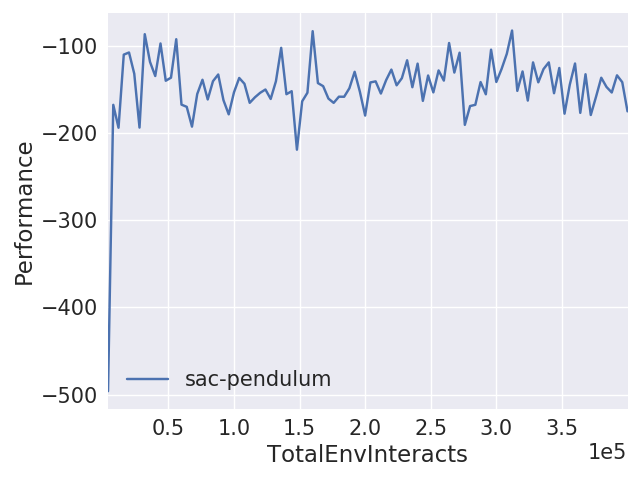
\includegraphics[width=\textwidth]{figures/rl-framework/sac-pendulum.png}
         \caption{Pendulum-v0 (Very Easy)}
     \end{subfigure}
     \hfill
     \begin{subfigure}[t]{0.32\textwidth}
         \centering
         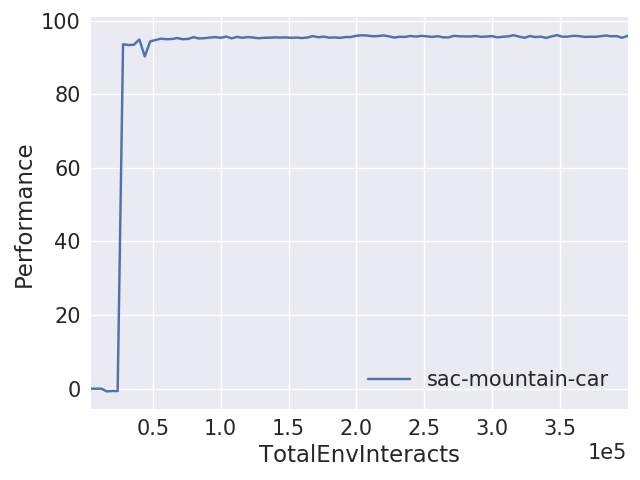
\includegraphics[width=\textwidth]{figures/rl-framework/sac-mountain-car.png}
         \caption{MountainCarContinuous-v0 (Easy)}
     \end{subfigure}
     \hfill
     \begin{subfigure}[t]{0.32\textwidth}
         \centering
         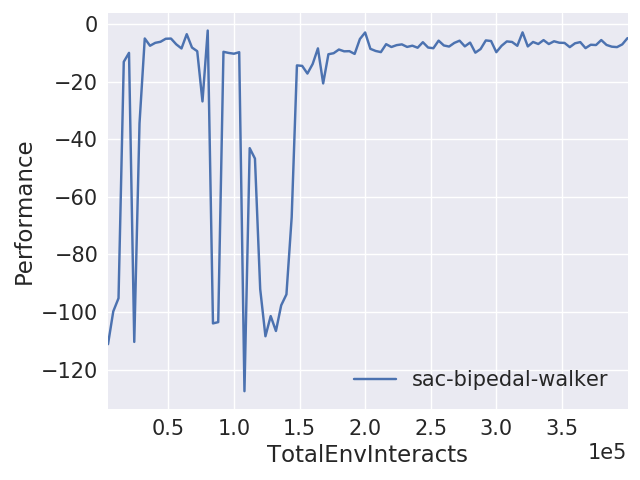
\includegraphics[width=\textwidth]{figures/rl-framework/sac-bipedal-walker.png}
         \caption{BipedalWalker-v3 (Hard)}
     \end{subfigure}
        \caption{Performance of Spinning Up implementation of SAC on different environments, using default parameters}
        \label{fig:spinup-SAC}
\end{figure}

Spinning Up implementation performs well and converges quickly on easy environments, but it provides disappointing results on the harder BipedalWalker-v3 environment. SAC is expected to have better exploration and achieve better results on BipedalWalker-v3 environment before 300.000 environment interacts \cite{gym-leaderboard}. But it never managed to escape a local minimum for a long period of training time. Considering our sailing environment will be pretty complex, Spinning Up implementation of SAC is not suitable for use on this project.

\subsection{RL Framework Features} \label{RLF:framework-features}

\begin{wrapfigure}{r}{0.4\textwidth}
\vspace{-4em}
\centering
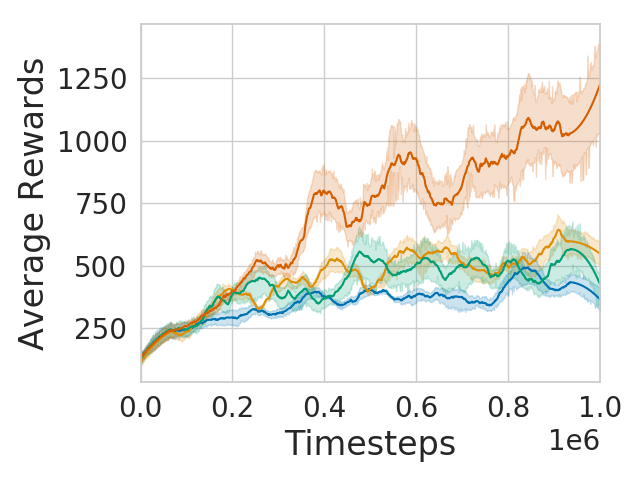
\includegraphics[width = 0.39\textwidth]{figures/rl-framework/hyperparameter-ddpg.png}
\caption{DDPG on Walker2d-v1 with random hyperparameters \cite{hyperparameter-ddpg}}
\label{fig:hyperparameter-ddpg}
\vspace{-1em}
\end{wrapfigure}

Spinning Up Framework lacks some important features for Reinforcement Learning. First, it does not support continuing training of a previously trained agents. This is problematic in a few ways: it costs precious time and resources to train agents from scratch every time, plus even if models are trained again from ground up, no two reinforcement learning runs will be identical because of the noise or stochasticity in the algorithms.

The second lacking feature is that there is no hyperparameter optimization support. Hyperparameters can cause huge difference in performance \cite{hyperparameter-ddpg}. A comparison of DDPG on Walker2d-v1 with random hyperparameters can be seen in Figure \ref{fig:hyperparameter-ddpg}. The best and worst performing hyperparameters have approximately 3-fold average reward difference after 1 million timesteps.

Both of these features, and probably more that will arise in the future are important for this project, so another framework with these additional features is needed.


\subsection{Stable Baselines 3}
Stable Baselines3 (SB3) is a library providing reliable implementations of state-of-the-art reinforcement learning algorithms in PyTorch, complete with a training framework 'RL Baselines3 Zoo' which contains scripts for training, evaluating agents, tuning hyperparameters, plotting results, and recording videos \cite{stable-baselines3}.

SB3 solves both of the problems of Spinning Up Framework mentioned in sections \ref{RLF:imp-diff} and \ref{RLF:framework-features}. SB3 is focused on providing reliable implementations that can be used on Deep Reinforcement Learning Research, instead of an education focus of Spinning Up. SB3 implementations are fully functional, high quality, and they match the results of best previous implementations. A performance comparison of Soft Actor Critic implementations of Stable Baselines3 and OpenAI Spinning Up can be seen in Figure \ref{fig:spinup-vs-sb3}. We are expecting SAC to converge to 300 score which is the goal of this environment \cite{Bipedal-Walker-v2} in around 300.000 steps \cite{gym-leaderboard}. Stable Baselines3 implementation delivers expected results whereas the Spinning Up implementation falls short. The hyperparamaters were tuned in SB3 implementations, but weren't tuned for Spinning Up as it doesn't support hyperparameter tuning.

\begin{figure}[h]
     \centering
     \begin{subfigure}[t]{0.49\textwidth}
         \centering
         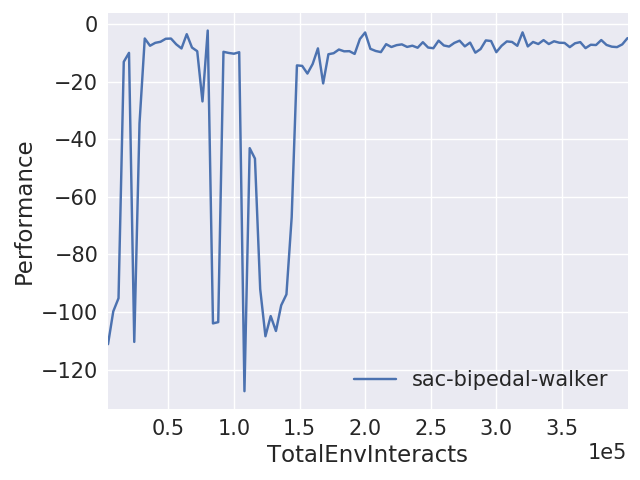
\includegraphics[width=0.91\textwidth]{figures/rl-framework/sac-bipedal-walker.png}
         \caption{Spinning Up implementation (Default parameters) - Goal not achieved in 400.000 steps}
     \end{subfigure}
     \hfill
     \begin{subfigure}[t]{0.49\textwidth}
         \centering
         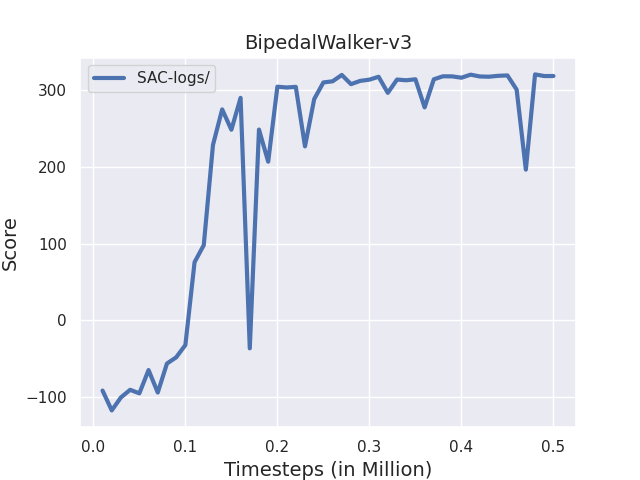
\includegraphics[width=\textwidth]{figures/rl-framework/sb3-sac-BipedalWalker-v3.png}
         \caption{Stable Baselines3 implementation (Tuned parameters) - Goal Achieved in 200.000 steps}
     \end{subfigure}
        \caption{Training Performance of SAC implementations. Goal Score: 300}
        \label{fig:spinup-vs-sb3}
\end{figure}

Moreover, the RL Baselines Zoo has the missing features of Spinning Up's training framework, namely hyperparameter optimization and continuing training of previously trained models \cite{rl-zoo3}. Therefore, SB3 will be the choice of RL Framework.

\section{Future Plans}

\qquad\textbf{State Estimator:} 
First, the state estimator concerns mentioned needs to be tackled. Details can be found in sections \ref{subsec:tack-detection-and-datasets} and \ref{subsec:data-split-methods}. For now, only the \emph{Atlantic} dataset that has the tack information available will be used to bypass the tack detection problem.
\begin{comment}
As for the Data Split concerns, if data leak is present and it considerably affects the performance of the models, revising the state estimator work might be required. Another further work not mentioned before is testing whether the state estimator is transferable to other boats it was not trained on. The transferability result does not affect the future plans, but is interesting to find out. 
\end{comment}
After the data split method is decided, the state estimator models that will be used on the Reinforcement Learning environment will be created.

\textbf{Gym Environment:}
In order to use Stable Baselines Zoo and Algorithms, our environment needs to implement the OpenAI Gym interface, and be structured as an importable PIP package. Using the state estimator models created, a Gym environment will be implemented. Several obstacles that are currently unknown are expected during this step.

\textbf{Hindsight Experience Replay}
(HER) is a technique that helps agents to learn from mistakes, which allows the agents to learn with sparse and binary rewards, therefore eliminating the need for complicated reward engineering \cite{her-paper}. While making environment creation easier, it also improves performance and sample efficiency. To use HER, our environment needs to implement the stricter GoalEnv interface, which inherits from the Gym interface.

\textbf{RL Algorithms:}
After the Gym environment is implemented, the RL algorithms can be tested on the new environment. The suggested algorithms to be trained are: SAC with HER, which is the current state of the art that is widely tested; plus TQC with HER, which is a recent advancement that shows promising results. All of these algorithms are available in Stable Baselines 3, although TQC is still in beta.

\textbf{RL Obstacles:} 
If there are no signs of life after training with tuned hyperparameters, reward engineering can be tried instead of using HER. Another concern is that the algorithms will learn a loophole in the state estimator models which is unrealistic but will make the boat go faster. If that becomes the case, early stopping before it happens, or revisiting the state estimator models might be needed.

\begin{figure}[h]
\centering
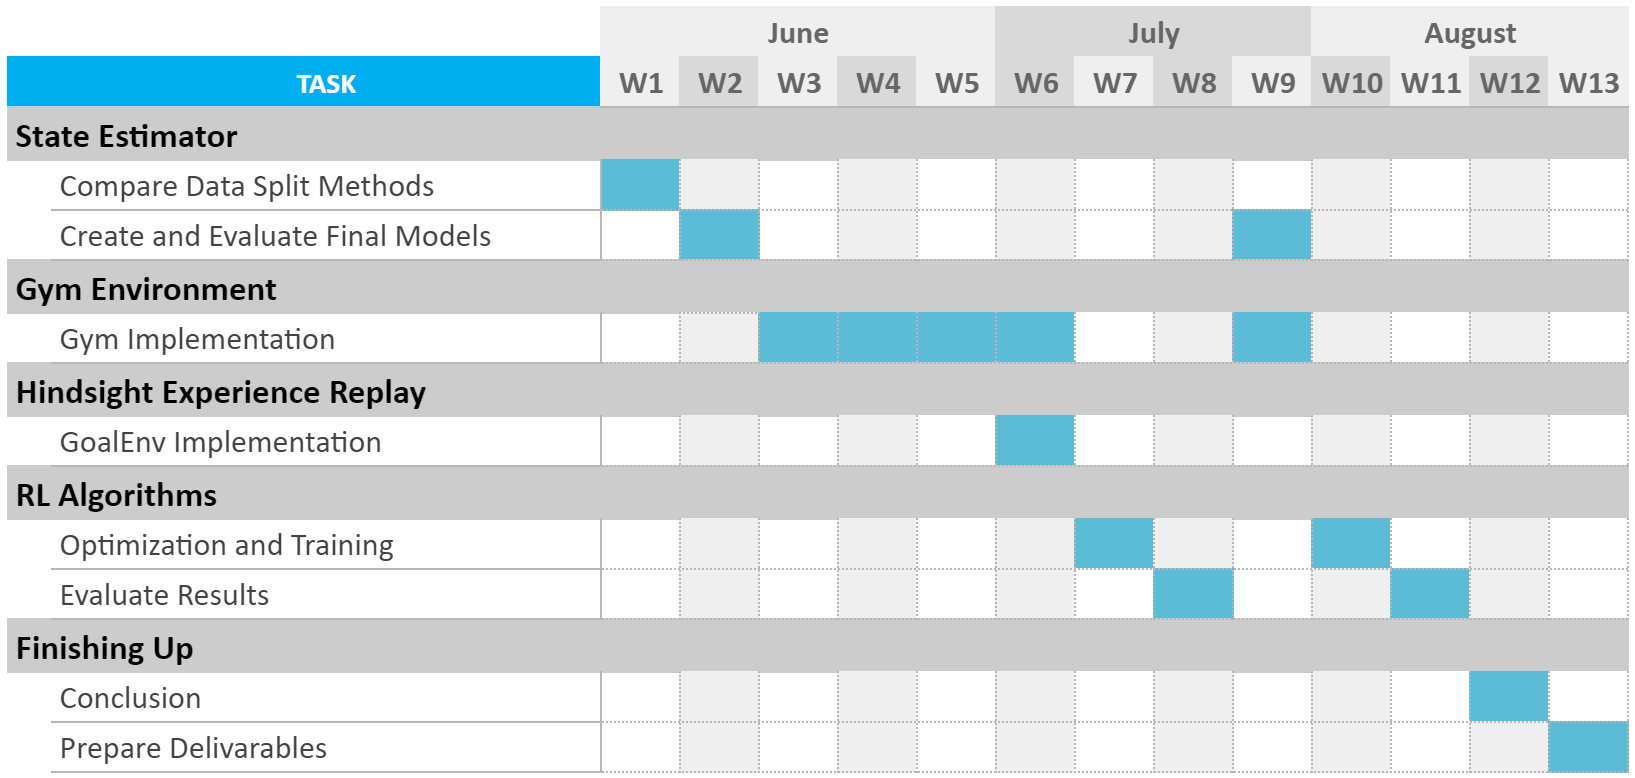
\includegraphics[width = 0.92\hsize]{figures/gantt-chart2.png}
\caption{Tentative timeline, including a second iteration for improvements}
\label{fig:gantt-chart}
\end{figure}
